\subsection{Problem 11}%
\label{sec:problem_11}
Generate the values of the polynomial $y = 40 + 10x + 5x^2 + 3x^3 + 2x^4 + x^5 + x^6$
for $x = 1, 2, \ldots, 14$.
First fit the polynomial $y = a_0 + a_1x + a_2x^2 + a_3x^3 + a_4x^4 + a_5x^5 + a_6x^6$
to the generated data in the LS sense and compare the estimated coefficients
$a_0, a_1, \ldots, a_6$ to the true ones.
Then perturb the observed data with an additive Gaussian noise $\it{N}(0,\sigma^2)$, and
illustrate the fitting error (the Euclidean norm) versus the standard deviation $\sigma$.
Estimate the maximal value of $\sigma$ for which fitting error does not exceed $10^{-6}$,
assuming double precision arithmetic operations.
%%%%%%%%%%%%%%%%%%%%%%%%%%%%%%%%%%%%%%%%%%%%%%%%%%%%%%%%%%%%%%%%%%%%%%%%%%%%%%%

%%%%%%%%%%%%%%%%%%%%%%%%%%%%%%%%%%%%%%%%%%%%%%%%%%%%%%%%%%%%%%%%%%%%%%%%%%%%%%% Recursive Least Squares

\subsubsection*{Exponentially Weighted Recursive Least Squares}
\begin{enumerate}
    \item \textbf{Parameter Vector Initialization:}
    \[ \hat{\theta} = \mathbf{0} \]
    where \( \hat{\theta} \) is the estimate of the parameter vector of length \texttt{param\_num}.
    
    \item \textbf{Error Covariance Matrix Initialization:}
    \[ P = 1000 \cdot I \]
    where \( I \) is the identity matrix of size \texttt{param\_num} $\times$ \texttt{param\_num}. This large initial value indicates high uncertainty in the initial parameter estimates.
    
    \item \textbf{Forgetting Factor:}
    \[ \lambda = 0.99 \]
    a value close to 1, indicating that recent observations are slightly more weighted than older ones.
\end{enumerate}

\subsubsection*{Recursive Update For Each Observation}

For each observation at time step \(i\), the algorithm updates the estimate of \( \hat{\theta} \) as follows:

\begin{enumerate}
    \setcounter{enumi}{4}
    \item \textbf{Regression Vector Construction:}
    The regression vector \( \phi_i \) is constructed for each observation, with \( \phi_{i,j} = x_i^{j-1} \) for \( j = 1, \ldots, \text{param\_num} \).
    
    \item \textbf{Error Covariance Matrix Update:}
    \[ P = \left( P - \frac{P \phi_i \phi_i^T P}{\lambda + \phi_i^T P \phi_i} \right) / \lambda \]
    
    \item \textbf{Kalman Gain Calculation:}
    \[ K = P \phi_i \]
    
    \item \textbf{Parameter Estimate Update:}
    \[ \hat{\theta} = \hat{\theta} + K \left( y_i - \phi_i^T \hat{\theta} \right) \]
\end{enumerate}

\subsubsection*{Mathematical Representation}

Used Exponentially Weighted Recursive Least Squares algorithm is represented as follows:

\begin{enumerate}
    \item Initialize:
    \[ \hat{\theta} = \mathbf{0}, \quad P = 1000 \cdot I, \quad \lambda = 0.99 \]
    
    \item For each observation \(i\) from 1 to \(n\):
    \begin{itemize}
        \item[a.] Construct \( \phi_i \) with \( \phi_{i,j} = x_i^{j-1} \).
        \item[b.] Update \( P \):
        \[ P = \left( P - \frac{P \phi_i \phi_i^T P}{\lambda + \phi_i^T P \phi_i} \right) / \lambda \]
        
        \item[c.] Compute \( K \):
        \[ K = P \phi_i \]
        
        \item[d.] Update \( \hat{\theta} \):
        \[ \hat{\theta} = \hat{\theta} + K \left( y_i - \phi_i^T \hat{\theta} \right) \]
    \end{itemize}
\end{enumerate}

This algorithm recursively updates the parameter estimates \( \hat{\theta} \) based on new observations \( (x_i, y_i) \), adjusting the estimate to minimize the error between the model predictions and the observed data. The key feature of RLS is its ability to adapt the estimates as new data arrives, with the forgetting factor \( \lambda \) moderating the influence of older observations on the current estimate.

\subsubsection*{Mathematics}
\subsubsection*{Calculating $\sigma$ for given fitting error}
To analytically find $\sigma$ value for defined fitting error of $10^{-6}$, first would be redefinition of our regression model
\[
    y = a_0 + a_1 x + a_2 x^2 + a_3 x^3 + a_4 x^4 + a_5 x^5 + a_6 x^6 + \epsilon
\]
where \(\epsilon\) is the term denoting Gaussian noise \(N(0, \sigma^2)\).\\
In next step the design matrix \(A\) for the polynomial regression, which includes terms for \(x, x^2, \ldots, x^6\).\\
With observed points in \(x = 1, 2, \ldots, 14\), this matrix becomes a Vandermonde matrix.\\
The least squares estimation of the coefficients, \(\hat{a}\), in matrix form is given by:
\[
    \hat{a} = (A^T A)^{-1} A^T b
\]
The influence of noise \(\epsilon\) on the estimation is reflected in the covariance matrix which is under the influence of noise \(\epsilon\) is:
\[
    \text{Cov}(\hat{a}) = \sigma^2 (A^T A)^{-1}
\]
Each element of this matrix represents the variance of the corresponding coefficient due to noise.

\textbf{Objective:}
Solve for \(\sigma\) such that the Euclidean norm of the difference between the original coefficients and those estimated from noisy data equals \(10^{-6}\). Formally:
\[
    \sqrt{\sum_{i=0}^6 (a_i - \hat{a}_i)^2} = 10^{-6}
\]

\subsubsection*{Calculation Steps}
Each coefficient's variance can be extracted from the covariance matrix:
\[
    \text{Var}(\hat{a}_i) = \sigma^2 (A^T A)^{-1}_{ii}
\]
Assuming the noise affects each coefficient independently, the sum of squared differences due to noise is:
\[
    \sum_{i=0}^6 \sigma^2 (A^T A)^{-1}_{ii} = 10^{-12}
\]
This equation arises from setting the Euclidean norm squared of the difference (the sum of squares) to \(10^{-12}\), reflecting that the total error in terms of the Euclidean norm is \(10^{-6}\).

By rearranging given equation we are able to solve for \(\sigma\):
\[
    \sigma = \sqrt{\frac{10^{-12}}{\sum_{i=0}^6 (A^T A)^{-1}_{ii}}}
\]
Denominator is the trace of \((A^T A)^{-1}\), which sums the variances across all coefficients.\\
By using MATLAB calculated $\sigma$ value is $\approx 8.86*10^{-8}$.

%%%%%%%%%%%%%%%%%%%%%%%%%%%%%%%%%%%%%%%%%%%%%%%%%%%%%%%%%%%%%%%%%%%%%%%%%%%%%%%
%%%%%%%%%%%%%%%%%%%%%%%%%%%%%%%%%%%%%%%%%%%%%%%%%%%%%%%%%%%%%%%%%%%%%%%%%%%%%%%
\subsubsection*{Solution}
Generated curves for approximations of polynomial 
\begin{figure}[H]
    \centering
    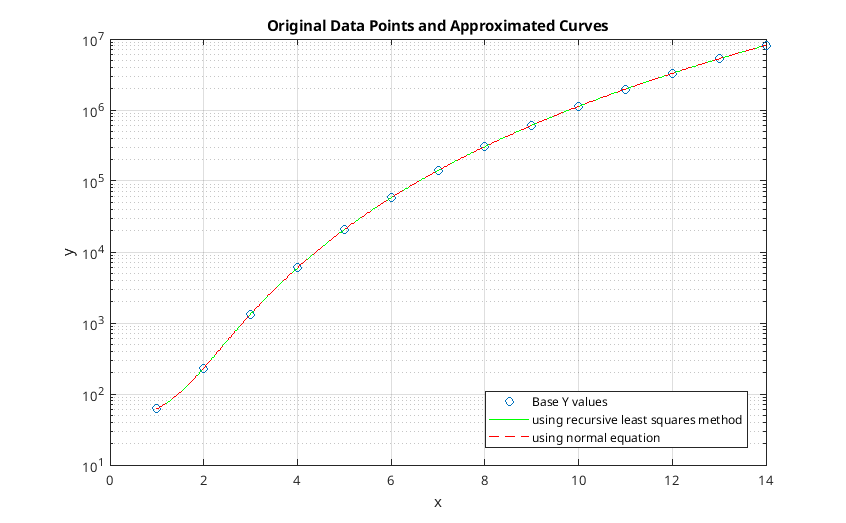
\includegraphics[width=1\textwidth]{images/Problem_11/ApproxCurves.png}
    \caption{Approximations of polynomial using Normal equation and Recursive Least Squares method}
\end{figure}
During the programming of fitting error calculation, we weren't able to get such low values for fitting error. 
It's possible that our method for calculating fitting error was incorrect, or used methods had awful stability.
For $\sigma \in (0:0.0001:0.1)$ our lowest error was with the use of normal equation at $1.0953*10^-5$.
\begin{figure}[H]
    \centering
    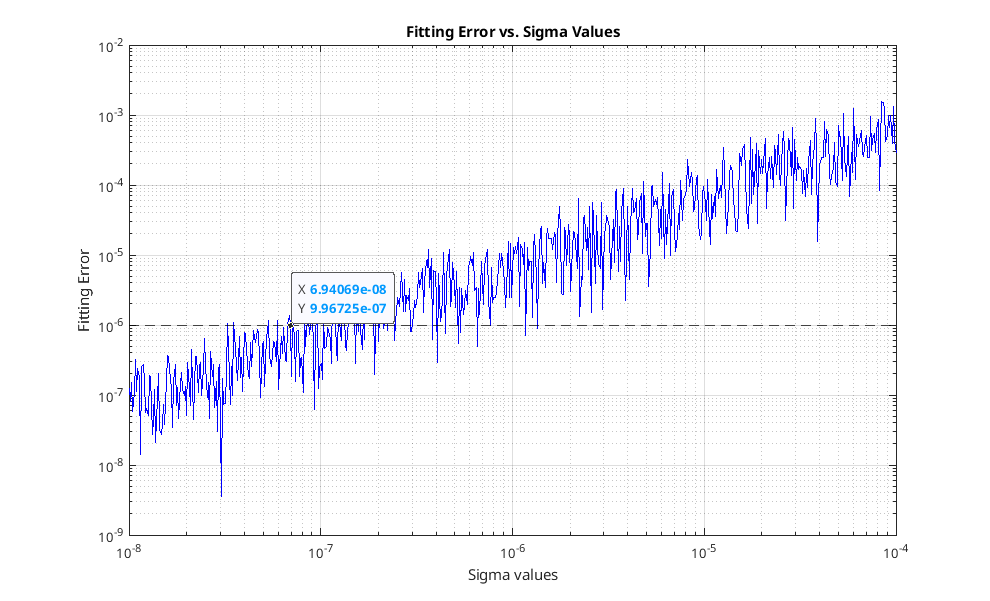
\includegraphics[width=1\textwidth]{images/Problem_11/fittingErrors.png}
    \caption{Fitting errors of approximations Normal equation and RLS with perturbed input data set}
\end{figure}
Weighted recursive least squares method had higher fitting error than normal equation.
%%%%%%%%%%%%%%%%%%%%%%%%%%%%%%%%%%%%%%%%%%%%%%%%%%%%%%%%%%%%%%%%%%%%%%%%%%%%%%%
